\chapter{مروری بر مطالعات انجام شده}\label{chap:literature_review}
  \thispagestyle{empty}
  \section{مقدمه}
  \section{پردازش مه و پردازش لبه}
    واژه‌ی اینترنت اشیاء برای اولین بار توسط کوین اشتون\LTRfootnote{Kevin Ashton} در یک ارائه برای استفاده از بازشناسی با امواج رادیویی\LTRfootnote{RFID} در مدریت زنجیر تأمین\LTRfootnote{Supply Chain} استفاده شد\cite{shton2009that}.
    اینرنت اشیاء امکان اتصال هر کسی در هر مکان و زمانی به هر چیزی در هر مکانی و هر زمانی را فراهم می‌کند.
    با پیشرفت تکنولوژی به سمت جامعه‌ای پیش می‌رویم که همه افراز و همه‌ی اشیاء متصل خواهند بود\cite{zheng2011internet}.
    ایده‌ی اصلی اینترنت اشیاء این است که امکان اتصال خودکار و امن و انتقال داده‌ بین دستگاه‌های فیزیکی و برنامه‌های کاربردی را فراهم می‌کند.
    در واقع اینرنت اشیاء این امکان را ایجاد می‌کند که اشیاء فیزیکی بتوانند ببینند، بشنوند، و با صحبت کردن با یکدیگر بتوانند تصمیم‌گیری کنند و کار‌هایی را انجام دهند\cite{al2015internet}.
    در طول زمان انتظار می‌رود اینرنت اشیاء کاربرد‌های خانگی و تجاری فراوانی داشته باشد، کیفیت زندگی افراد را بهبود ببخشد و باعث رشد اقتصاد جهانی بشود.

    گسترش اینترنت اشیاء و موفقیت سرویس‌های ابری باعث ایجاد الگو‌ی جدیدی در پردازش داده‌ها به نام پردازش لبه \LTRfootnote{Edge Computing} شده‌است.
    در این الگوی پردازشی سعی بر این است که پردازش داده‌ها در لبه شبکه انجام شود.
    طبق براورد‌های انجام شده \cite{2018cisco} تعداد دستگاه‌های متصل شده به شبکه ۵۰ میلیارد عدد خواهد بود.
    بعضی از کاربردهای اینترنت اشیاء نیاز به زمان پاسخ کوتاه دارند، بعضی دارای داده‌های ممکن است دارای داده‌های محرمانه وشخصی باشند و و بعضی از این کاربرد‌ها می‌توانند بار سنگینی برای شبکه داشته باشند و پردازش ابری ممکن است روش مناسبی برای این کاربرد‌ها نباشد.

    \subsection{چرا به پردازش لبه نیاز داریم؟}
      در حال حاظر نرخ تولید داده در لبه شبکه در حال افزایش می‌باشد.
      بنابر این پردازش این داده‌ها در لبه شبکه روش کارامدتری خواهد بود.
      در ادامه دلایلی برای لزوم استفاده از پردازش لبه را بر می‌شماریم \cite{shi2016edge}:
      \begin{description}
        \item [فشار از سمت پردازش ابری]
          قرار دادن همه وظایف پردازش در ابر به عنوان یک روش کارآمد برای پردازش داده‌ها شناخته شده است چرا که قدرت پردازشی ابر قابل مقایسه با قدرت پردازشی اشیاء در لبه شبکه نیست.
          با این حال، در مقایسه با پیشرفت سریع سرعت پردازش داده‌ها، پهنای‌باند شبکه‌ها تقریبا ثابت مانده‌اند.
          افزایش تولید داده در لبه شبکه باعث شده است که انتقال این داده‌ها به گلوگاه پردازش ابری تبدیل شود.
          به عنوان نمونه یک هواپیما‌ی بویینگ ۷۸۷ در یک ثانیه ۵ گیگابایت داده تولید می‌کند در صورتی که پهنای‌باند بین هواپیما و ایستگاه زمین به اندازه‌ی ارسال این حجم از داده نمی‌باشد.
          یک اتومبیل خودران را به عنوان نمونه‌ای دگیر در نظر بگیرید.
          در هر ثانیه ۱ گیگابایت داده توسط آن تولید می‌شود و نیاز به پردازش بلادرنگ\LTRfootnote{Real-Time} این داده‌ها برای تصمیم گیری درست نیاز است.
          اگر قرار باشد که همه این داده‌ها برای پردازش به ابر فرستاده‌شوند، زمان پاسخ بسیار طولانی خواهد بود.
          علاوه بر این پهنای باند و قابل اطمینان شبکه‌های فعلی برای پردازش داده‌‌های تعداد زیادی خودرو در یک منطقه کافی نخواهد بود.
          در این موارد داده‌ها باید در لبه شبکه پردازش شوند.
          این کار زمان پاسخ کوتاه‌تر، پردازش کارآمد‌تر و فشار کم‌تر بر شبکه را به ارمغان می‌آورد.

        \item [کشش از سمت اینترنت اشیاء]
          همانطور که قبلا بیان شد، می‌توان در نظر گرفت که تعداد اشیاء لبه شبکه میلیارد‌ها دستگاه برسد.
          در نتیجه داده‌های خام تولید شده توسط آن‌ها حجم بسیار بزرگی خواهند داشت و این حجم بزرگ باعث می‌شود که روش‌های مرسوم پردازش ابری مناسب برای پردازش این حجم از داده‌ها نباشند.
          در نتیجه می‌توان درنظر گرفت که بیشتر این داده‌های تولید شده در اینترنت اشیاء هیچ وقت برای پردازش به ابر ارسال نمی‌شوند و در لبه شبکه پردازش می‌شوند.

          \cref{fig:chapter_2:cloud_paradigm} ساختار مرسوم در پردازش ابری را نشان می‌دهد.
          تولید کننده‌های داده، داده‌های خام را به ابر انتقال می‌دهند.
          مصرف کننده‌ها هم با ارسال درخواست نتیجه را از ابر بدست می‌آورند.
          با این حال این ساختار برای استفاده در اینترنت اشیاء مناسب نیست.
          اولا حجم داده‌ی تولید شده در لبه شبکه بسیار زیاد است که پهنای باند شبکه و منابع پردازشی زیادی را طلب می‌کند.
          ثانیا حفظ حریم شخصی به عنوان یک مانع برای پردازش ابری ایجاد می‌کند.
          در انتها، بسیاری از گره‌های انتهایی در اینترنت اشیاء دارای انرژی محدودی هستند و ماژول‌های مخابرات بی‌سیم معمولا مصرف انرژی بالایی نیاز دارند.
          در نتیجه انجام وظایف پردازشی در لبه شبکه می‌تواند از لحاظ مصرف انرژی بهینه‌ باشد.

          \begin{figure}[h]
            \centerline{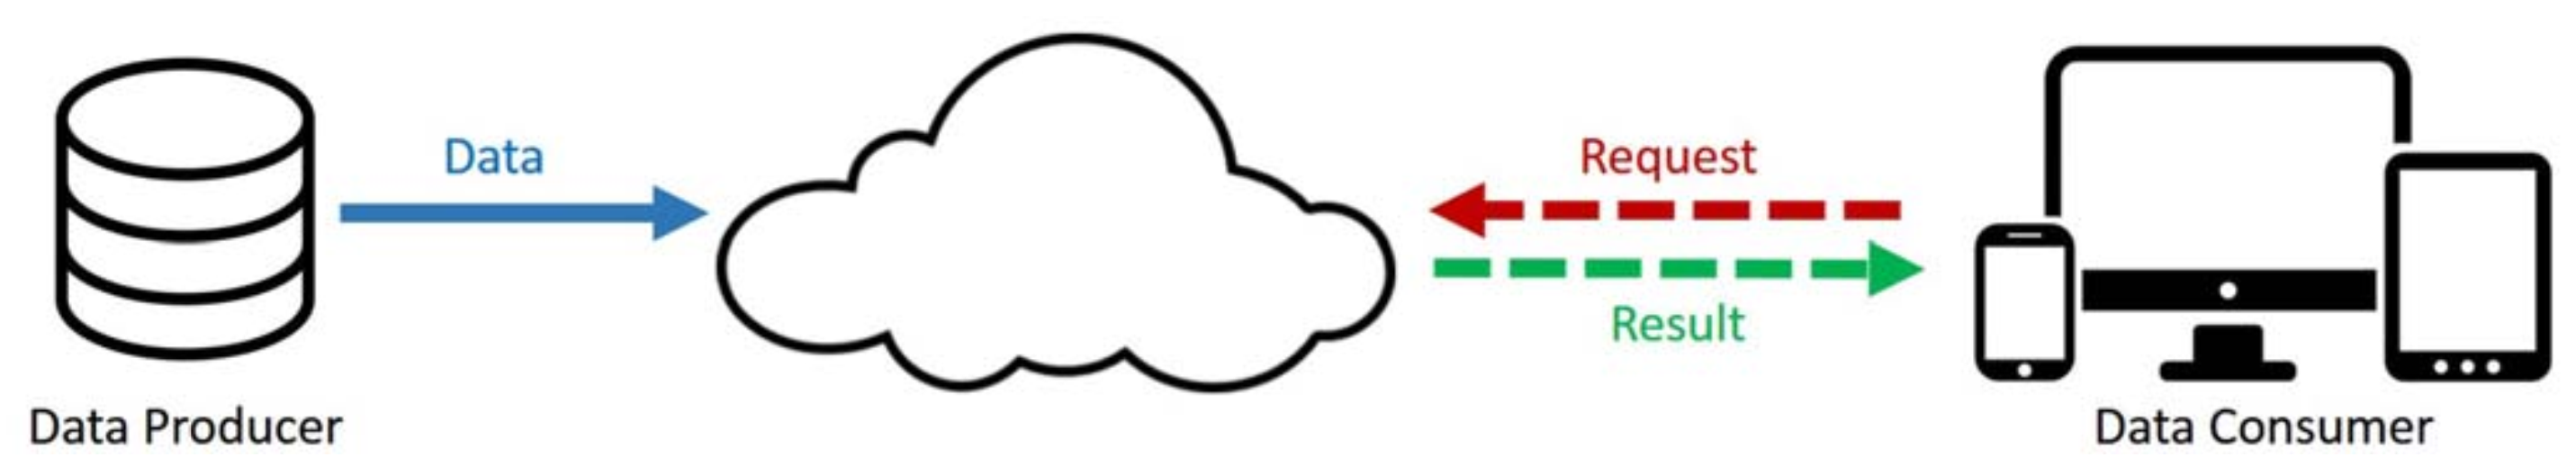
\includegraphics[width=10cm]{graphics/chapter_2/cloud_paradigm}}
            \caption{الگوی پردازش ابری \cite{shi2016edge}}
            \label{fig:chapter_2:cloud_paradigm}
          \end{figure}

        \item [تغییر از مصرف کننده داده به تولید کننده داده]
          در الگوی پردازش ابری، دستگاه‌های انتهایی در لبه شبکه معمولا نقش مصرف کننده داده را دارند.
          به عنوان نمونه می‌توان تماشای یک ویدیو را مثال زد.
          با این حال امروزه مردم در حال تولید داده توسط دستگاه‌هایشان هستند.
          برای مثال امروزه بسیار عادی است که افراد عکس‌ها و ویدیو‌هایی که توسط خودشان ضبط شده است را در سرویس‌های اینترنتی مختلف به اشتراک بگذارند.
          در \cite{2019domo} اشاره شده است که در هر دقیقه در \lr{twitter} ۵۱۱۲۰۰ توییت جدید ارسال می‌شود و در \lr{instagram} ۵۵۱۴۰ عکس جدید بارگذاری می‌شود.
          باید توجه داشت که این تصاویر و ویدیوها می‌توانند حجم زیادی داشته باشند و پهنای باند زیادی را برای بارگذاری استفاده کنند.
          در این موارد ویدیو‌ها باید ابتدا حجمشان در لبه شبکه کاهش پیدا کند تا به وضوح تصویر\LTRfootnote{resolution} مناسب برای بارگذاری در شبکه برسند.
          به عنوان نمونه‌ی دیگر می‌توان دستگاه‌های مربوط به سلامت را مثال زد.
          داده‌های جمع‌آوری شده توسط این دستگاه‌ها معمولا خصوصی است و پردازش این داده‌ها در لبه شبکه به جای ارسال داده‌ها برای پردازش به ابر به حفظ حریم خصوصی افراد کمک می‌کند.

      \end{description}
    
    \subsection{پردازش لبه چیست؟}
      پردازش لبه به همه تکنولوژی‌هایی اطلاق می‌شود که امکان انجام پردازش‌ها در لبه شبکه را فراهم می‌کنند.
      در اینجا منظور از لبه، همه منابع پردازشی و شبکه ای است که بین منبع داده‌ها (جایی که داده‌ها در آن جا تولید می‌شوند) و مراکز داده‌ی ابری قرار دارند.
      برای مثال یک دروازه‌ی شبکه در یک خانه هوشمند، می‌تواند یک منبع پردازشی لبه بین اشیاء و مرکز داده‌ی ابری باشد یا یک مرکز داده‌ی کوچک، می‌تواند یک منبع پردازشی لبه بین دستگاه‌های سیار و ابر در نظر گرفته شود.
      منطق در پردازش لبه این است که پردازش داده‌ها باید در همسایگی منبع داده‌ها انجام شود.
      با این منطق پردازش لبه و پردازش مه\cite{} دو مفهوم یکسان را خواهند داشت با این تفاوت که پردازش لبه تمرکزش سمت اشیاء است ولی پردازش مه تمرکزش سمت زیرساخت است.

      \begin{figure}[h]
        \centerline{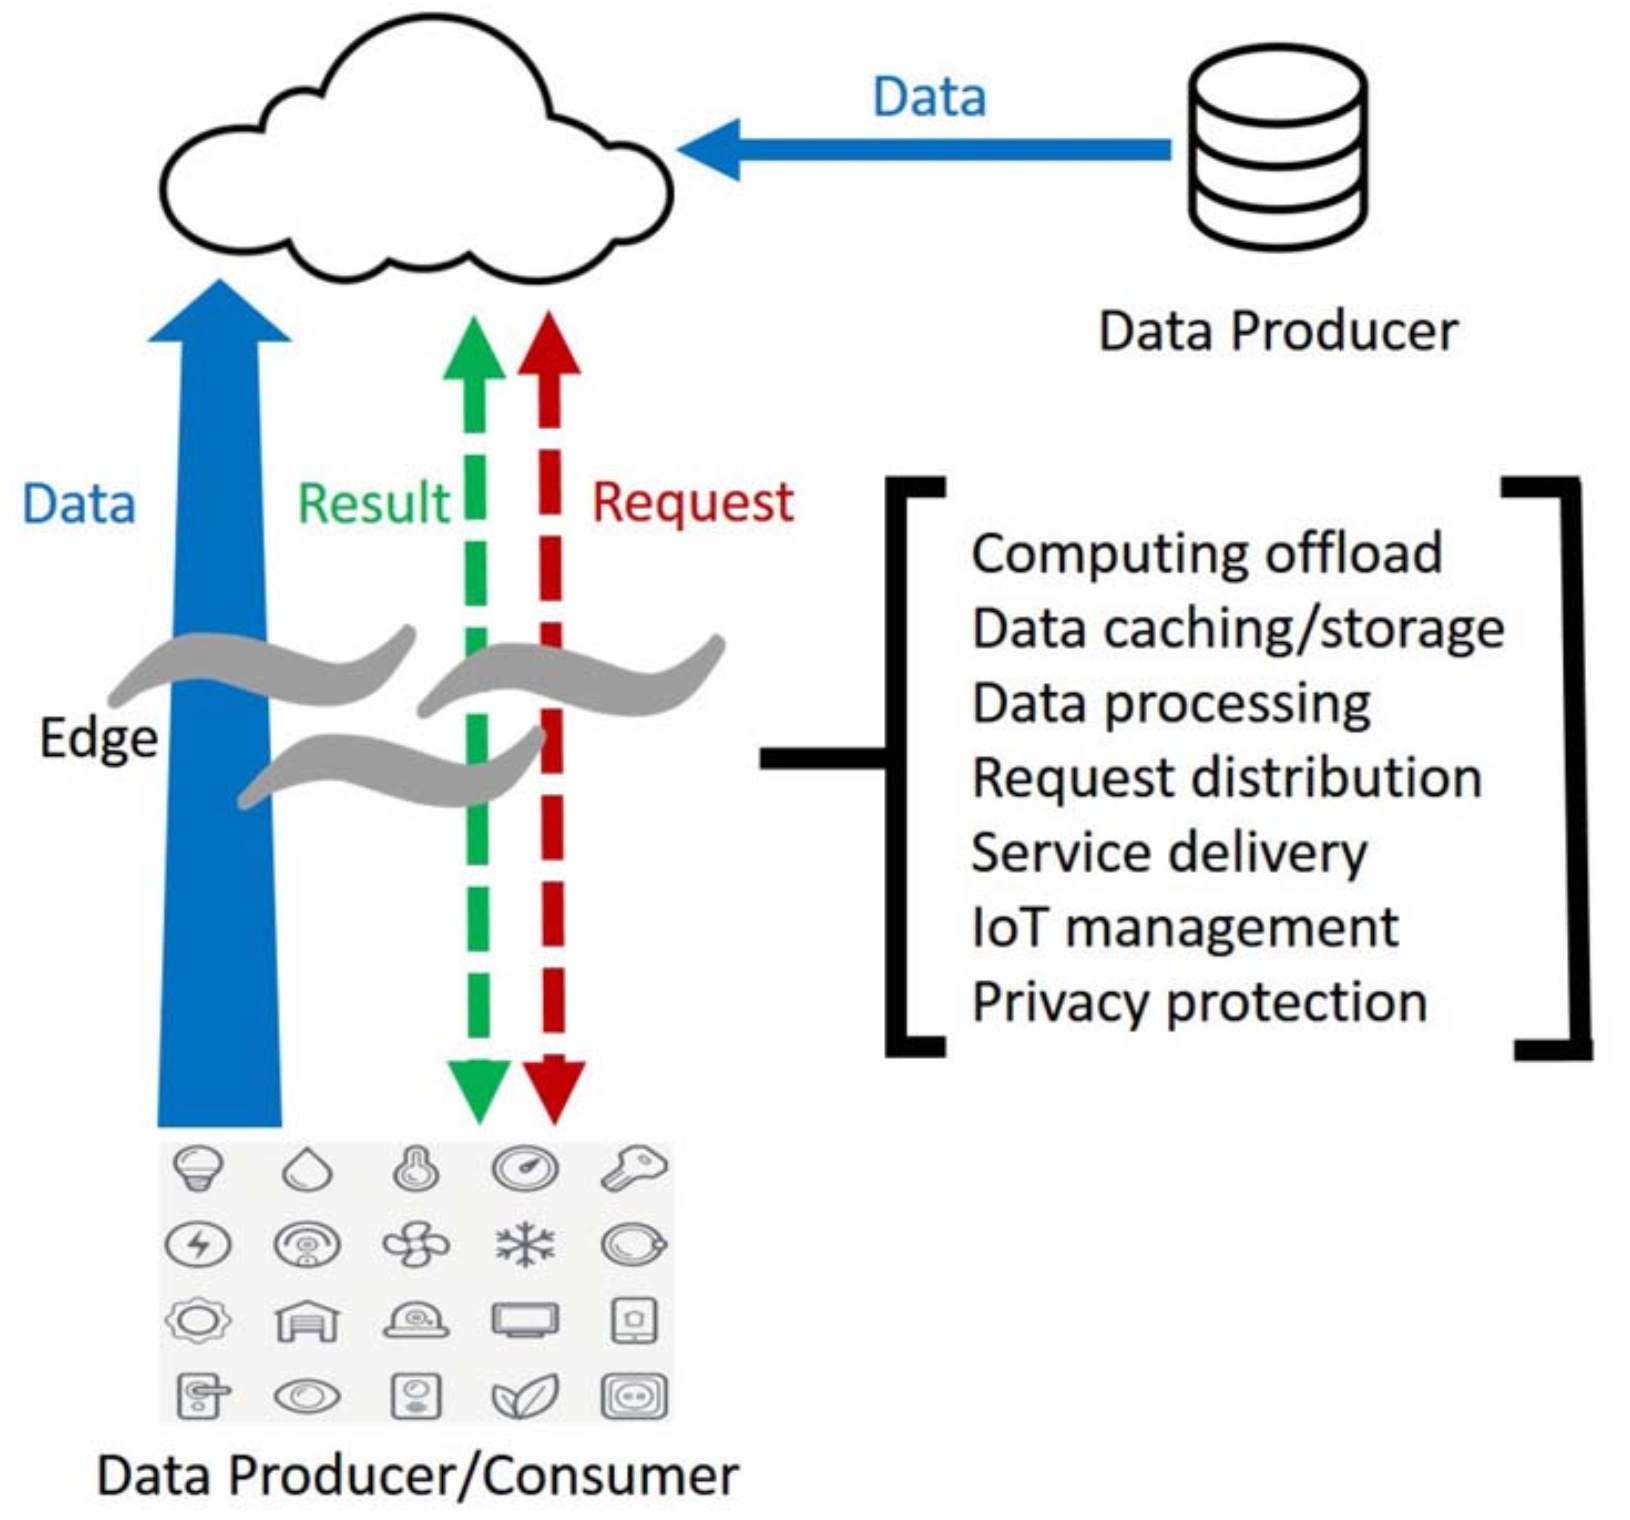
\includegraphics[width=10cm]{graphics/chapter_2/edge_paradigm}}
        \caption{الگوی پردازش لبه \cite{shi2016edge}}
        \label{fig:chapter_2:edge_paradigm}
      \end{figure}
      
      \cref{fig:chapter_2:edge_paradigm} جریان پردازش دو طرفه را در پردازش مه نشان می‌دهد.
      در الگو پردازش لبه، اشیاء نه تنها مصرف کننده داده بلکه تولید کننده‌ داده نیز هستند.
      در واقع در لبه اشیاء نه تنها می‌توانند سرویس و محتوا از ابر  درخواست نمایند بلکه می‌توانند وظایف پردازشی را هم انجام دهند.

    \subsection{مزایای پردازش لبه}